% This document is the template I use when building out resumes when friends or
%   family ask for help. It tends to have a complete-enough quality to it, that
%   allows for specializing, or enhancing sections when needed, but is
%   generally sufficient using just the base template.
% The content in the template is meant to be nothing more than a format-aware
%   Lorem Ipsum. In places where short lists were needed, they were used, and
%   silly content, or generally nonsensical content was used, as long as the
%   format of the content fit with expectations of that section.
\documentclass[pdftex,letterpaper,10pt]{article}

\usepackage[bottom=3.25cm, top=3.25cm, left=2.0cm, right=2.0cm]{geometry}
\usepackage{fancyhdr}
\usepackage{graphicx}
\usepackage{hyperref}
\usepackage[inline]{enumitem}

\usepackage{resume}

\def\EmailAddress{name@domain.tld}
\def\PhoneNumber{555-555-5555}
\def\Name{Firstname Lastname}

\newcommand{\GitHubHeader}{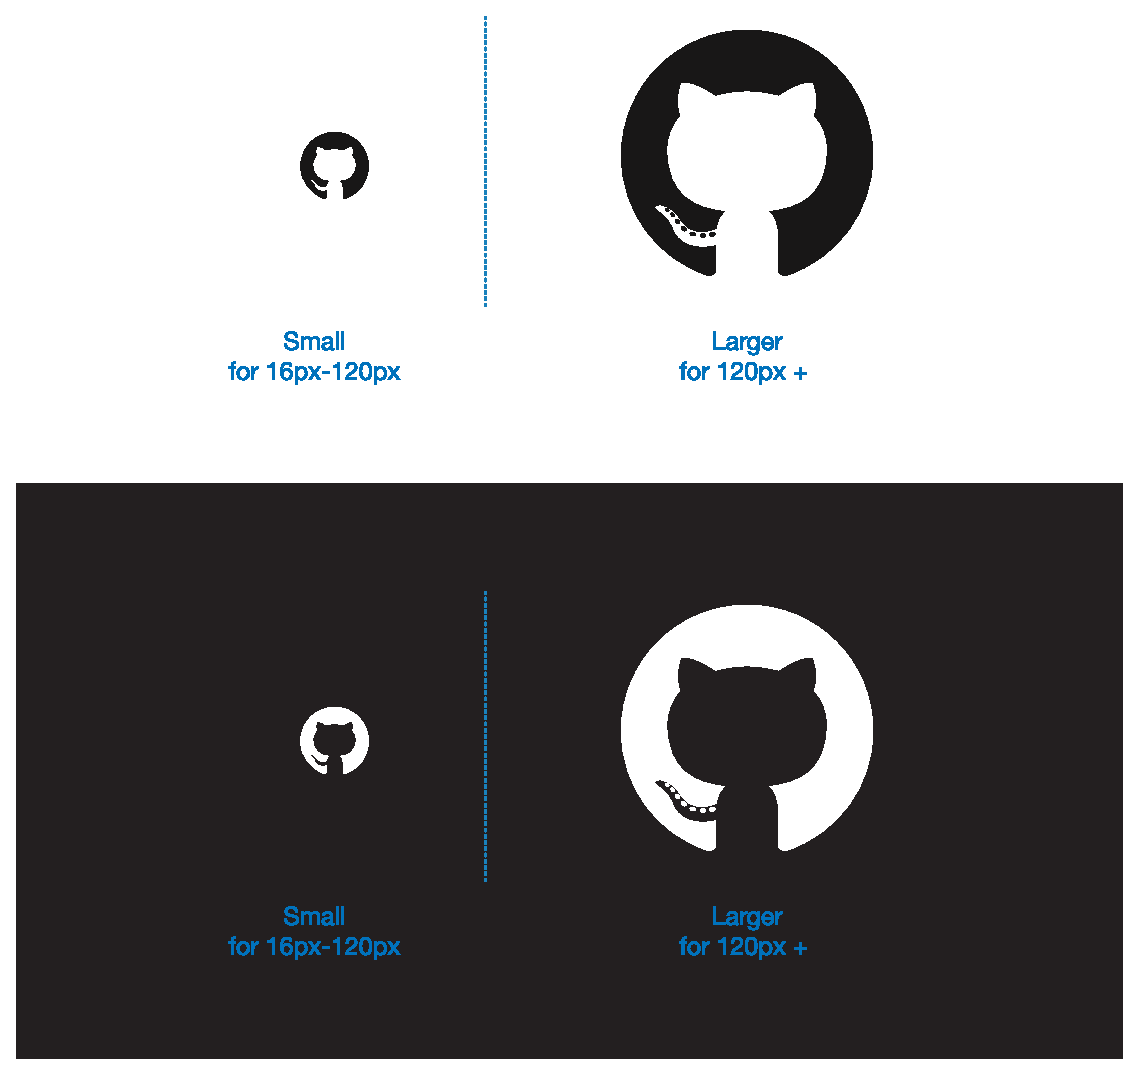
\includegraphics[clip,trim=4.8cm 14.55cm 12.75cm 1.95cm,scale=0.5]{img/GitHub-Mark.eps}}
\newcommand{\LinkedInHeader}{
\includegraphics[scale=0.4]{img/In-Black-0p5in-TM.eps}}


\usepackage[bitstream-charter]{mathdesign}
\usepackage[T1]{fontenc}

\fancyhead[L]{\href{mailto:\EmailAddress}{\EmailAddress}}
\fancyhead[C]{\huge \bfseries \Name}
\fancyhead[R]{\href{tel:\PhoneNumber}{\PhoneNumber}}

\fancyfoot[C]{}

\pagestyle{fancy}

% Headers for below the main header line
\newcommand{\LeftSubheader}{%
    \href{https://github.com/\GitHubUsername}%
        {\raisebox{-.25\height}{\GitHubHeader} GitHub/\GitHubUsername}%
}
\newcommand{\CenterSubheader}{\Address}
\newcommand{\RightSubheader}{%
    \href{https://www.linkedin.com/in/\LinkedInUsername}%
        {\raisebox{-.25\height}{\LinkedInHeader} LinkedIn/\LinkedInUsername}%
}

% Specifically asked for by the compiler, likely because of how tall everything
%   in the frame already is. Only really dictates the minimum height from the 
%   top margin.
\setlength{\headheight}{25pt}

% \cvtrue
\renewcommand{\baselinestretch}{1.15}
\renewcommand{\headrulewidth}{1.25pt}

\begin{document}%
%
\MakeSubheader%
%
\ifcv
\subsection*{Core Skills and Competencies}
\begin{skilltabular}
    General Skills  & Cooking, Cleaning, Organization \\
    Speaking Skills & Fast talking, Slow talking, Chipmunk talking, Foreign accents, Talking under my breath, Shouting, Whining like a baby \\
    Others          & Eating lots of food all at once, Sleeping for 20 hours straight
\end{skilltabular}
\fi
%
\subsection*{Work Experience}
\begin{job}{Ministry of Silly Talks}
    \begin{position}{Talk Master}{June 2014 - Present}
        \item Talked to many unique individuals, mimicking their accents.
        \item Engaged in numerous speaking competitions on behalf of the company, winning dozens of prizes over the course of a few years, and earned top-speaker awards from the company itself.
        \item Convinced many high ranking individuals that I was a distinguished individual by using the right voices.
    \end{position}
    \begin{position}{Talk Instructor}{May 2013 - May 2014}
        \item Designed training documentation for onboarding new talkers.
        \item Trained juniors how to talk silly talks.
        \ifcv
        \item Helped other instructors create lesson plans for group session, and one on one sessions.
        \fi
    \end{position}
\end{job}
%
\begin{job}{Sleep Center}
    \begin{position}{Junior Sleeper}{August 2012 - May 2013}
        \item Slept for 32 consecutive hours, when it was required to meet a quota from upper management.
        \ifcv
        \item Worked with in-house tools and processes to sleep on a day to day basis.
        \fi
    \end{position}
    \ifcv
    \begin{position}{Sleep Intern}{January 2012 - May 2012}
        \item Learned about Sleep Center's process for managing workflows, and worked on designing new sleep workflows.
        \item Complete internship with a rating of ``Fantabulousticulous'', the highest rating available from The University of Earth.
    \end{position}
    \else
    \justposition{Sleep Intern}{January 2012 - May 2012}
    \fi
\end{job}
%
\subsection*{Other Experience}
\begin{description}
    \item[Sleep] Although I do have professional experience sleeping, it is also a hobby of mine.
        I have been sleeping as a hobby for most of my professional life.
    \item[Silly Talks] A lot of my professional career has revolved around speaking, so on the side, I've also become somewhat of a silly-talker.
        Although I don't have any professional experience as a deep-talker, it is something that I've got a lot of experience in, and can hold my own in a deep-talk-off.
    \item[Management] Although the experience doesn't come from a professional setting, I manage a guild in the recent hit game Talk Mania X.
        I rally individuals from around the world to talk together 5 times a week so we can defeat the evils of silence.
\end{description}
%
\subsection*{Education}
\begin{school}{University of Earth}
    \begin{degree}{Msc. Talk Sciences}{2014 - 2016}
        \item Research projects included ``Life'' and ``More Life''
    \end{degree}
    \begin{degree}{BSc. Talk Sciences}{2010 - 2014}
        \item Graduated top of class of 7 billion.
    \end{degree}
\end{school}
%
\subsection*{Personal Interests}
\begin{itemize*}[itemjoin=\hspace{8pt},label={\(\bullet\)\hspace{2pt}}]
    \item Window shopping on \href{http://treadmills.com}{treadmills.com}, and \href{http://beds.com}{beds.com}
    \item Drinking water with my best friends on Saturdays in the rain
    \item Setting up special programs on my treadmill to allow me to do the silliest of walks without needing any kind of professional stage to practice at home
\end{itemize*}
%
\end{document}
